\documentclass[letterpaper,addpoints,answers]{exam}
\usepackage{graphicx}

\newcommand{\hide}[1]{%
}

\begin{document}

%\pagestyle{headandfoot}
%\lhead{
  %\large\bfseries Physics 107\\ 
  %Midterm Exam, June 15, 2009
%}
%\chead{}
%\rhead{
  %\large\bfseries Name:\enspace\makebox[2in]{\hrulefill}\\
  %\large\bfseries Signature:\enspace\makebox[2in]{\hrulefill}
%}
%\lfoot{}
%\cfoot[]{Page \thepage}
%\rfoot{}

\begin{coverpages}
 \large\bfseries
 
 \noindent 
 Physics 252: Electronics
 
 \vspace{2ex}
 \noindent
 Midterm Exam: February 26, 2013

 \vspace{5ex}
 \noindent 
 Name:\enspace\makebox[2in]{\hrulefill}\\

 \vspace{5ex}
 \noindent 
 This test is administered under the rules and regulations of the honor 
 code of the College of William \& Mary.  

 \vspace{5ex}
 \noindent 
 Show your work, and circle your answers.

 \vspace{5ex}
 \begin{center}
  \gradetable[v][questions]
 \end{center}
\end{coverpages}
 

\begin{questions}

\question

Consider the loaded voltage divider shown below.
\begin{center}
 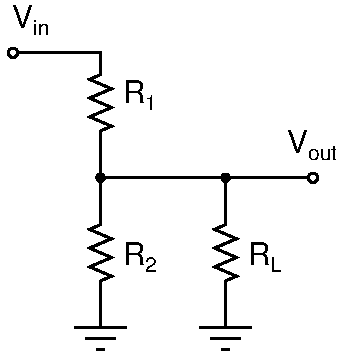
\includegraphics[width=0.25\textwidth]{./schematics/loaded_voltage_divider}
\end{center}
\begin{parts}
 \part[10]
  What must be the value of the load resistor $R_L$ to ensure maximum power transfer to
  it if $R_1 = 2\,\hbox{k}\Omega$ and $R_2 = 8\,\hbox{k}\Omega$?

  Answer: Maximum power transfer occurs when the load resistance is equal to the Th\'evenin
  resistance of the voltage divider, $R_L = R_{1||2} = 1.6\,\hbox{k}\Omega$.
  
  \vskip 1in
 \part[10]
  At the point of the maximum power transfer to the load resistor $R_L$, what
  is the value of the current passing through the resistor $R_1$
  if $V_{in} = 10\,\hbox{V}_{DC}$?

  Answer: Since the load resistance is equal to the Th\'evenin resistance, the output voltage $V_{out}$ is half of the Th\'{e}venin voltage $V_{Th} = \frac{R_2}{R_1 + R_2} V_{in} = 8$\,V.  This means that the voltage across resistor $R_1$ is $V_{in} - \frac{1}{2} V_{Th} = 6$\,V.  The current through resistor $R_1$ is then $6\,\hbox{V} / 2\,\hbox{k}\Omega = 3\,\hbox{mA}$.
  
  \vskip 1in
\end{parts}


\pagebreak

\question

You are hired as a research assistant for an electronics lab. Your first
assignment is to characterize a black box (which seems to be a power
supply) given to you.

In a nearby lab book you find a series of measurements on this box.
In particular you find the voltage drop across several load resistors
connected to the box (see the table below).

\begin{center}
 \begin{tabular}{|c|c|}
  \hline
   $R_L$         &  $V_L$ \\ 
  \hline
   1\,k$\Omega$  &  10\,V \\
   100\,$\Omega$ &  2\,V  \\
  \hline
 \end{tabular}
\end{center}
 
\begin{parts}
 \part[10]
  Find the equivalent Th\'{e}venin voltage and resistance of this black box. 
  
  Answer: The Th\'evenin voltage is $V_{Th} = V_L + R_{Th} I_L = V_L + R_{Th} V_L / R_L$.  This
  gives us two equations, which we can subtract to find $0 = (10\,\hbox{V} - 2\,\hbox{V}) + 
  R_{Th} (10\,\hbox{mA} - 20\,\hbox{mA})$.  We solve for $R_{Th}$ and find $R_{Th} = 800\,\Omega$,
  and then $V_{Th} = 18\,\hbox{V}$.

  \vskip 2in
\end{parts}


\pagebreak

\question

For the circuits shown below specify if it is a low-pass, high-pass, band-pass or band-reject filter.

{\bf Hint:} It may be useful to think about the transfer function at high and low frequencies.
\begin{parts}
 \part[2] Circle one: band-pass \quad \emph{low-pass} \quad high-pass \quad band-reject
 \begin{flushleft}
 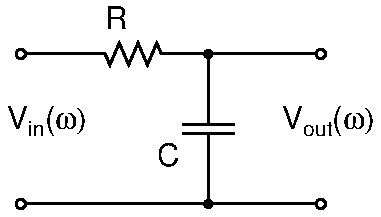
\includegraphics[height=0.7in]{./schematics/rc_low_pass}
 \end{flushleft}

 \part[2] Circle one: band-pass \quad low-pass \quad \emph{high-pass} \quad band-reject
 \begin{flushleft}
 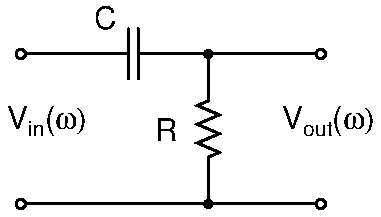
\includegraphics[height=0.7in]{./schematics/rc_high_pass}
 \end{flushleft}

 \part[2] Circle one: band-pass \quad low-pass \quad \emph{high-pass} \quad band-reject
 \begin{flushleft}
 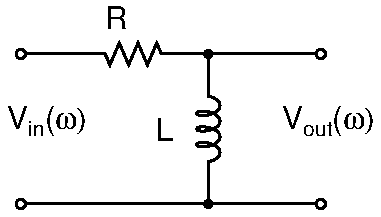
\includegraphics[height=0.7in]{./schematics/rl_high_pass}
 \end{flushleft}

 \part[2] Circle one: band-pass \quad \emph{low-pass} \quad high-pass \quad band-reject
 \begin{flushleft}
 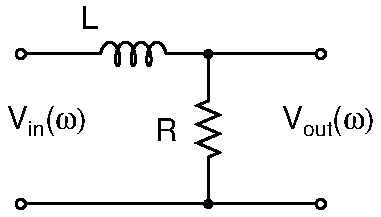
\includegraphics[height=0.7in]{./schematics/rl_low_pass}
 \end{flushleft}

 \part[4] Circle one: band-pass \quad low-pass \quad high-pass \quad \emph{band-reject}
 \begin{flushleft}
 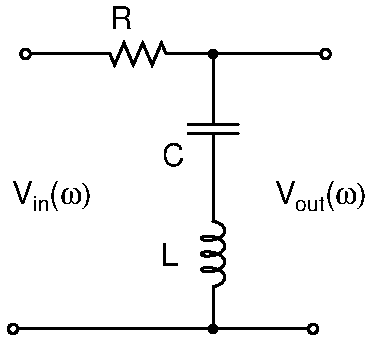
\includegraphics[height=1.1in]{./schematics/rlcnotch}
 \end{flushleft}

 \part[4] Circle one: \emph{band-pass} \quad low-pass \quad high-pass \quad band-reject
 \begin{flushleft}
 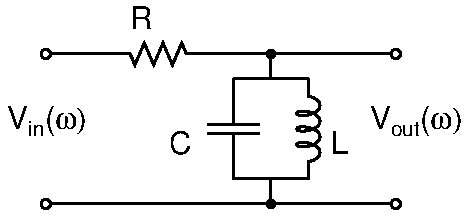
\includegraphics[height=0.7in]{./schematics/rlc_band_pass}
 \end{flushleft}

 \part[4] Circle one: \emph{band-pass} \quad low-pass \quad high-pass \quad band-reject
 \begin{flushleft}
 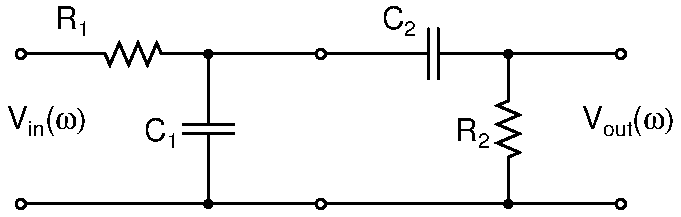
\includegraphics[height=0.7in]{./schematics/band_pass_filter}
 \end{flushleft}
\end{parts}

 
\pagebreak

\question

Consider the filter shown below.
\begin{center}
 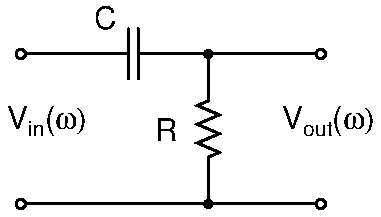
\includegraphics[width=0.25\textwidth]{./schematics/rc_high_pass}
\end{center}
\begin{parts}
 \part[5]
  What is the absolute value of the gain of this filter as a function of $\omega$?

  Answer: The gain is $G(\omega) = \frac{R}{R + 1/j \omega C} = \frac{j \omega RC}{1 + j \omega RC}$,
  and the absolute value is $|G(\omega)| = \frac{\omega RC}{\sqrt{1 + \omega^2 R^2 C^2}}$.  This does
  indeed go to 0 when $\omega \to 0$ and to 1 when $\omega \to \infty$.
 \part[5]
  Sketch the Bode plot of the absolute value of the gain of this filter.

  Answer:
  \begin{center}
   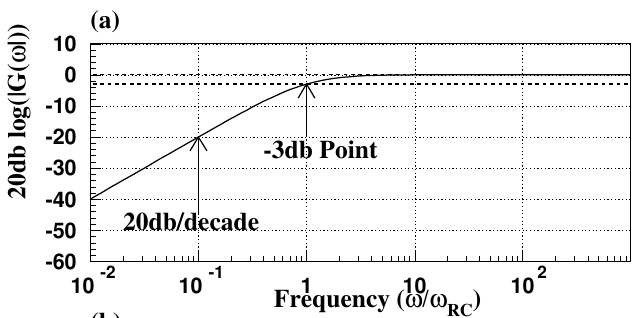
\includegraphics[width=0.5\textwidth]{./pics/rc_high_pass_bode}
  \end{center}
 \part[10]
  Find the average power dissipated by the resistor if the amplitude of the input
  signal is $V_{in} = 1\,\hbox{V}$, $R = 1\,\hbox{k}\Omega$,
  $C = 10\,\hbox{nF}$, and $\omega = \omega_{RC}$.
  
  Answer: The power dissipated in the resistor is $p(t) = v(t)^2 / R$.  The average power is then
  $P_{avg} = V_{RMS}^2 / R = V_{out}^2 / 2 R$ with amplitude $V_{out} = |G(\omega_{RC})| V_{in} = 1 / \sqrt{2}\,\hbox{V}$.
  The average power dissipated then $P_{avg} = 0.25\,\hbox{mW}$.
 \part[10]
  At the same conditions as above, find the average power dissipated by the capacitor?

  Answer: Ideal capacitors do not dissipate power.
\end{parts}


\pagebreak

\question

Your experimental apparatus generates useful signals at a frequency $f_s = 10$\,kHz 
with an amplitude $V_s = 0.1$\,V.  Unfortunately extremely strong noise couples
at a frequency $f_n = 0.1$\,kHz with an amplitude $V_n = 10$\,V.

During this problem you can use approximations and the simplified transfer
function representation.

\begin{parts}
 \part[5]
  What is the signal to noise ratio (SNR) coming from the apparatus?  Express your
  answer in either linear or dB scale, but be clear about which one you use.
  
  Answer: $SNR = V_s/V_n = 0.01 = -40\,\hbox{dB}$.
 \part[5]
  In a rush to improve the quality of the signal (i.e. SNR) you search
  through the lab and find a low-pass RC filter with $f_{3dB} = 1$\,kHz.

  What is the SNR at the output of this filter? Is it a good filter for the job?
  
  Answer: The filter will not suppress the 0.1\,kHz noise, but suppress the 10\,kHz signal
  by a factor 10, or 20\,dB.  The SNR becomes now 0.001 or -60\,dB.  This is not a good filter.
 \part[10]
  If it is up to you to design a filter, what kind of filter would you
  use?  Where would you place the $f_{3dB}$ of your filter for these
  noise conditions?  Draw a schematic of your filter.  What is the
  SNR after your improved filter?

  Answer: We should use a high pass filter, and try to suppress the noise as much as possible
  while keeping the signal strength.  This is achieved by placing $f_{3dB}$ at 10\,kHz.  The
  signal is not suppressed but the noise, two decades down, is suppressed by 100, or -40\,dB.
  The SNR becomes 1, or 0\,dB: the signal and noise have the same strength.
  \begin{center}
   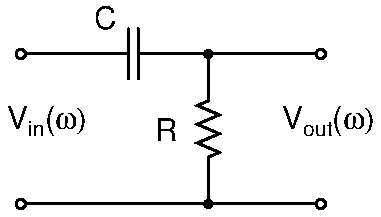
\includegraphics[width=0.25\textwidth]{./schematics/rc_high_pass}
  \end{center}
\end{parts}

\end{questions}

\end{document}
